\subsection{Leveraging a new architectural pattern}

\cite{czaplicki_elm:_2012} presented Elm, a new programming language that focuses on building purely functional graphical user interfaces. The language has evolved since then and managed to build an active community of users who primarily build web applications with it. While the community of Elm developers was growing, and more and more applications were developed with it, a specific pattern has been discovered. What today is widely called The Elm Architecture, or MVU for Model-View-Update outside of the Elm ecosystem, "seems to emerge naturally in Elm. Rather than someone 'inventing' it, early Elm programmers kept discovering the same basic patterns in their code." (\cite{czaplicki_elm_2018}).

\begin{figure}[H]
\centering
\caption{The MVU Architectural Pattern}
\label{fig:chasm}
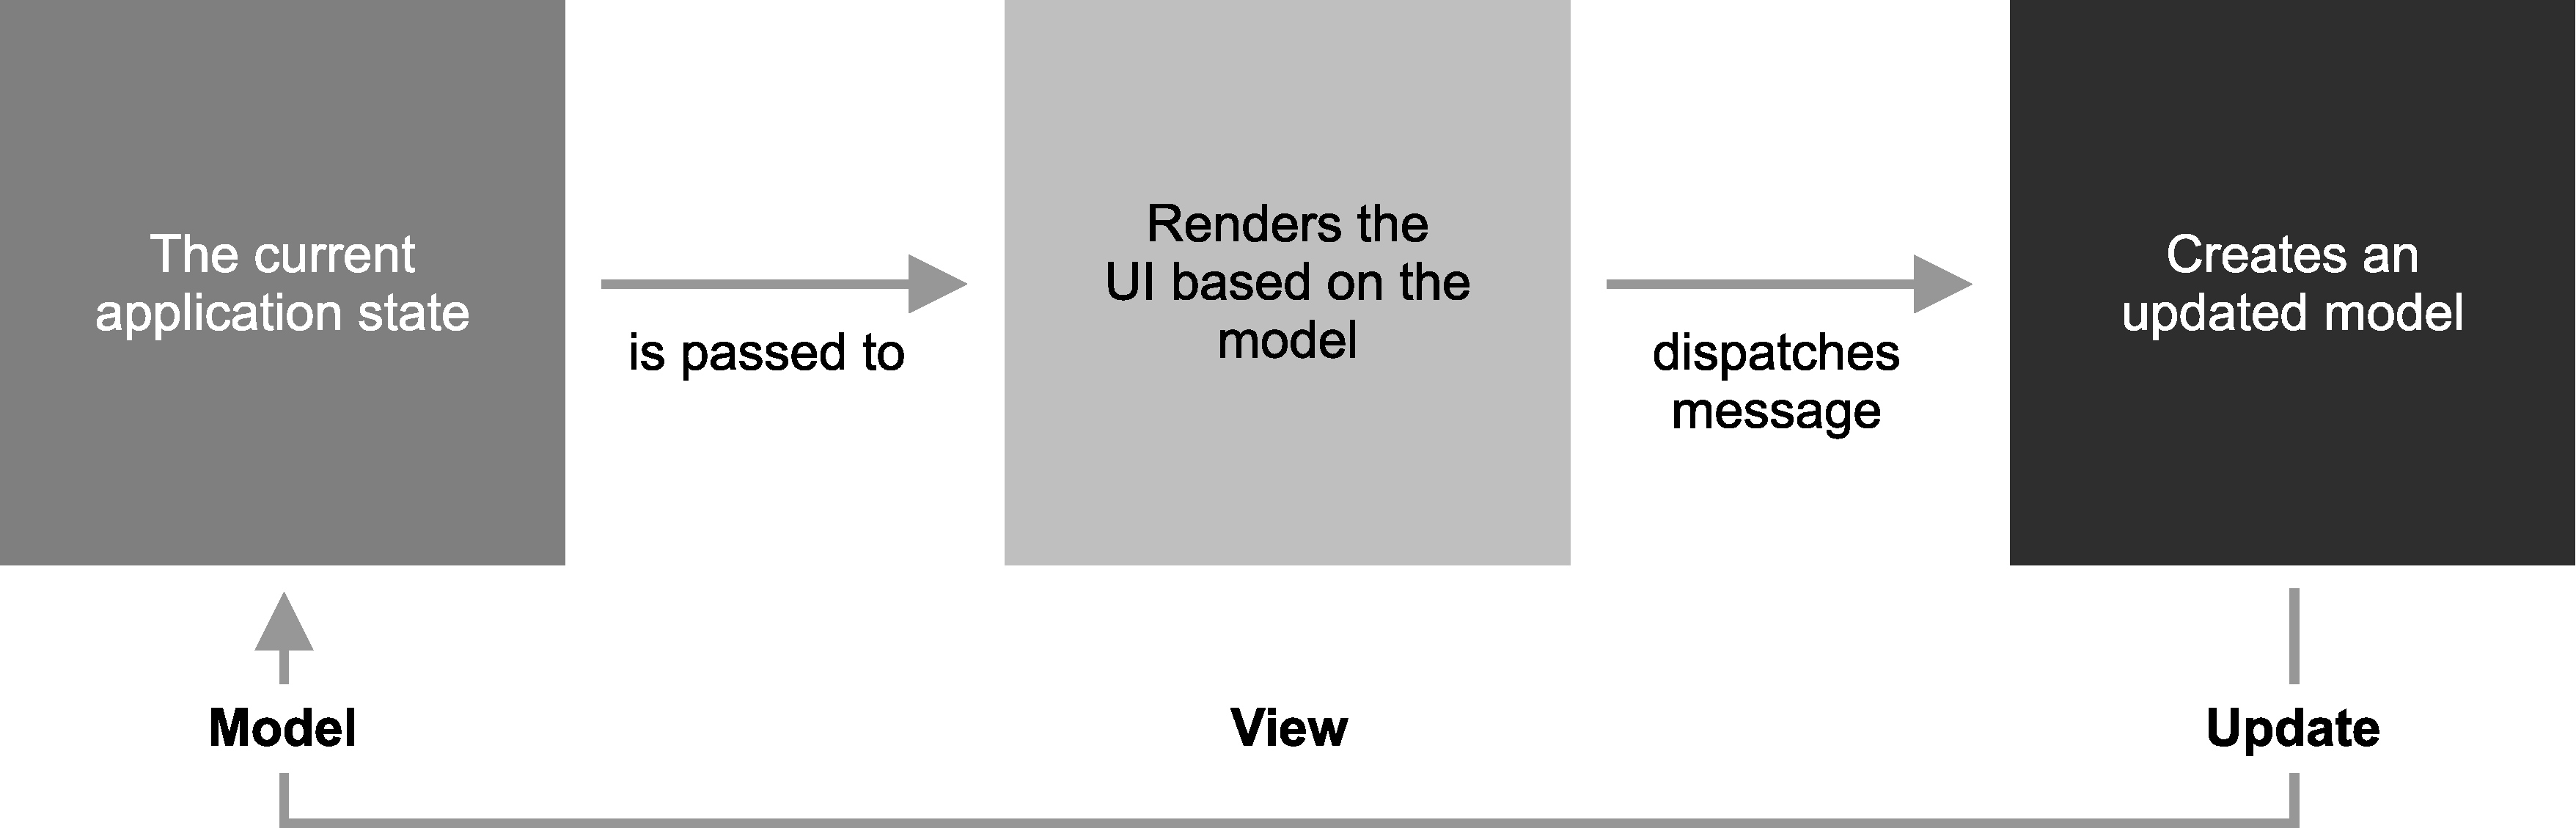
\includegraphics[width=\textwidth]{mvu}
\source{Own illustration}
\end{figure}

MVU has since been part of a movement towards architectures supporting unidirectional dataflows for user interfaces (\cite{staltz_unidirectional_2015}).

Unlike other architectural patterns like MVVM, "the Model" in MVU does not stand for an unspecified set of services and utilities, but for a very specific data structure that contains the (whole) state of the application. This data structure is immutable.

For rendering the view, the model is passed to a view function that returns the UI based on that exact model. This function is pure, which makes it possible to unit-test it — something hard to achieve or even impossible in most alternative solutions and especially for XAML UIs.

Of course, users want to interact with the interface, so it is not static and needs to react to input. That is done through commands, which eventually dispatch messages which are then being processed by an update function.

Update functions are pure, too. They take in the current model and a message and return a modified (updated) copy of the model. The update is being performed based on the message. Whenever a message is being dispatched, and therefore a new model is being created by the update function, the view is being re-rendered.

All of this ensures that data flows only in one direction through the whole application. This makes it very easy to reason about the program, it makes its components testable, and it enables features like time-travel debugging (\cite{james_time_2014}). As \cite[121]{loder_web_2018} notes, this is made possible through much wiring that is automatically being done in the background: "This makes it a little bit difficult at first to understand what is going on, but once the concept is clear we see that it reduces code in our application significantly."

\textbf{Introducing Fabulous}

Thanks to Fable, JavaScript has been an attractive compilation target for F\# developers for many years. Consequently, in 2016, Eugene Tolmachev announced the first version of what he called Elmish: an implementation of MVU for Fable (\cite{tolmachev_cross-platform_2016}).

In 2018, Don Syme was working together with the Xamarin team in his role as a researcher at Microsoft Research, trying to find out if there was a way to make app development with Xamarin as compelling to F\# developers as it was to build web applications (\cite{syme_making_2018}).

The existing solutions did not convince Syme: XAML seemed complicated and even unnecessary to him, and all the MVVM approaches were based on mutable data. Inspired by Fable and Elmish, Syme focused his research on a solution that could deliver a developer experience that was comparably easy and functional-first. He eventually came up with a library called Fabulous\footnote{https://fsprojects.github.io/Fabulous/ (retrieved August 8, 2019)}, an open-source project which is not affiliated to Microsoft but developed by its community of volunteers. Fabulous allows building mobile applications in a functional way on top of Xamarin.Forms by offering two different flavors: "Full Elmish" and "Half Elmish."

\textbf{Full Elmish}

When choosing Full Elmish, the entire Xamarin application can be written in F\# following the original idea of The Elm Architecture:

\begin{listing}[H]
\caption{A Fabulous sample program}
\begin{minted}{fsharp}
type Model =  { Count : int }
type Msg = | Increment | Decrement 

let init () = { Count = 0; }, Cmd.none

let update msg model =
    match msg with
    | Increment -> { model with Count = model.Count + 1 }, Cmd.none
    | Decrement -> { model with Count = model.Count - 1 }, Cmd.none

let view (model: Model) dispatch =
    View.ContentPage(content = 
        View.StackLayout(children = [ 
            View.Label(text = sprintf "Current Count: %d" model.Count)
            View.Button(
                text = "Increment", 
                command = (fun () -> dispatch Increment))
            View.Button(
                text = "Decrement", 
                command = (fun () -> dispatch Decrement))]))
\end{minted}
\end{listing}

The sample shows an (almost) complete Fabulous program, including all essential parts: model, messages, and the three functions to initialize and update the model and to render the view.

The model, in this case, contains just a simple count property which is initialized to 0. There are precisely two operations that can be done with this app: depending on the intent, which is expressed by a message, a new model is being created through the update function, with the count property either increased by one or decreased by one.

The view function takes in the model and a dispatch function. This allows creating a hierarchy of view elements depending on the model. In this simple case, the model's count value is rendered as a label. By using the dispatch function, updates can be triggered when the user interacts with the app through pressing either the increment or the decrement button.

Fabulous supports almost all Xamarin.Forms elements, which can be used in its terse DSL to express the view in a very similar hierarchical way as it would be done traditionally through XAML. The key difference is that there are no bindings that react to changes inside of the view. 

However, the view is being re-evaluated as soon as the model changes. To provide adequate rendering performance, the evaluation of views is handled by Fabulous in a way that allows a developer to specify custom differential updates for specific scenarios. So not the whole (complex) view is being re-rendered all the time but only those parts that need to reflect a change (\cite{syme_making_2018}).

As defining UI in code quickly becomes a tedious process when every change would require a complete compilation and deployment cycle, Fabulous offers a mechanism it calls "Live Update"\footnote{https://fsprojects.github.io/Fabulous/Fabulous.XamarinForms/tools.html (retrieved August 8, 2019)}. Live Update will send changes made to the code to the device or simulator/emulator, where the code is then evaluated, and the app is being refreshed immediately.

What developers get for free with Fabulous is the ability to unit-test most of the critical parts of an app, as those parts are implemented as pure functions that do not have any side-effects. The view, for example, can be tested by passing a mocked model to it. This is a unique advantage of the architecture and the Fabulous library, something hardly possible with XAML.

Some operations need to involve side-effects, like loading data from a database, or making network requests. Those operations are implemented through commands. Both the \mintinline{fsharp}{init} and the \mintinline{fsharp}{update} function return a tuple containing the model and a command. If there is something else returned than \mintinline{fsharp}{Cmd.none}, that command is being executed by Fabulous. The command itself is implemented as a function that can take in any parameter and almost always returns a new message which will then be passed to the update function again. This way, the – unidirectional – message loop stays intact.

\textbf{Half Elmish}

Developers with a background in XAML and C\# may be reluctant to choose the Full Elmish approach, especially because of the view part. Half Elmish\footnote{https://fsprojects.github.io/Fabulous/Fabulous.StaticView/ (retrieved August 8, 2019)} offers a compromise: Views can still be created (or re-used from existing solutions) in XAML, while model and update function are being written in F\#, next to a view function that wires up the bindings (\cite{bennett_building_2018}). This way, existing knowledge and code can be transferred, and the transition from XAML + C\# to an application entirely written in F\# is being made more convenient.
